
\documentclass[border=10pt, 12pt]{standalone}
\usepackage[svgnames]{xcolor}
\usepackage{amsmath}
\usepackage{pgfplots}
\pgfplotsset{compat=newest}
\usepackage[sfdefault]{FiraSans}
\usepackage{FiraMono}
\renewcommand*\familydefault{\sfdefault}
\begin{document}
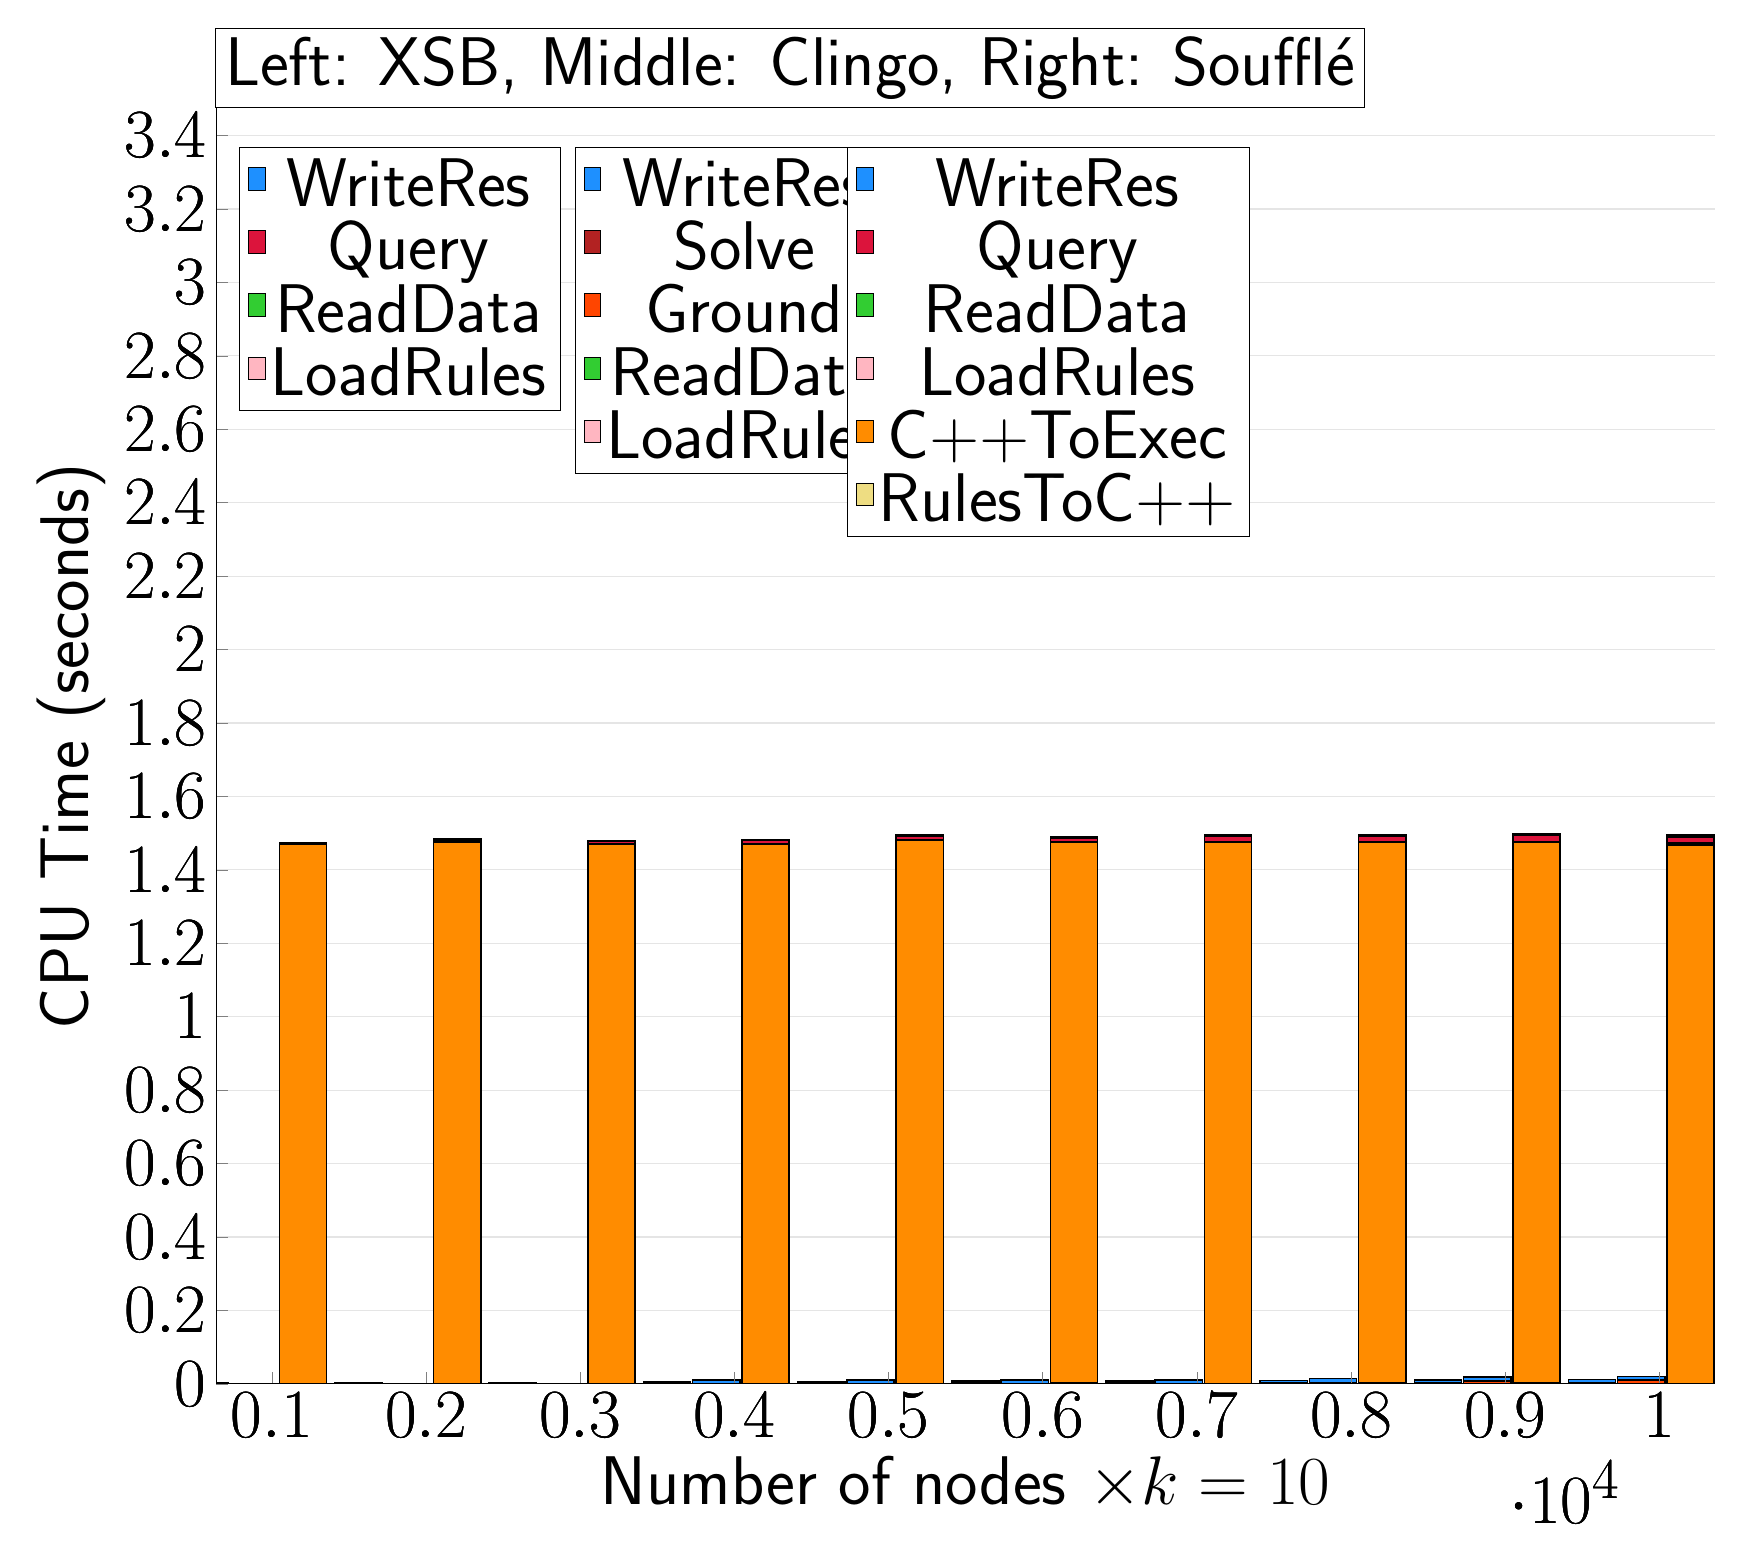
\begin{tikzpicture}
                        \begin{axis}[bar shift=-24.3pt, 
   ybar stacked,
   width=1.7\textwidth,
   bar width=0.6cm,
   ymajorgrids, tick align=inside,
   major grid style={draw=gray!20},
   xtick=data,
   ymin=0, ymax=3.474,
   axis x line*=bottom,
   axis y line*=left,
   enlarge x limits=0.04,
   legend style={
       at={(0.23, 0.97)},
       anchor=north east,
       legend columns=1,
       font=\Huge,
   },
   ylabel={CPU Time (seconds)},
   xlabel={Number of nodes $\times k=10$},
   label style={font=\Huge},
   tick label style={font=\Huge},
]
\addlegendimage{fill=DodgerBlue, draw=black, line width=0.2pt}
\addlegendentry{WriteRes}
\addlegendimage{fill=Crimson, draw=black, line width=0.2pt}
\addlegendentry{Query}
\addlegendimage{fill=LimeGreen, draw=black, line width=0.2pt}
\addlegendentry{ReadData}
\addlegendimage{fill=LightPink, draw=black, line width=0.2pt}
\addlegendentry{LoadRules}
\addplot +[fill=LightPink, draw=black, line width=0.55pt] coordinates {
(1000, 0.0005529999999999996)
(2000, 0.0005505999999999998)
(3000, 0.0005561999999999999)
(4000, 0.0005580000000000001)
(5000, 0.0005513999999999999)
(6000, 0.0005517999999999996)
(7000, 0.0005542000000000001)
(8000, 0.0005564)
(9000, 0.0005570000000000002)
(10000, 0.0005516)
};
\addplot +[fill=LimeGreen, draw=black, line width=0.55pt] coordinates {
(1000, 0.00020300000000000057)
(2000, 0.0002856000000000004)
(3000, 0.0003654000000000002)
(4000, 0.0004345999999999997)
(5000, 0.0005288000000000004)
(6000, 0.000609)
(7000, 0.0006742)
(8000, 0.0007702000000000007)
(9000, 0.0008243999999999998)
(10000, 0.0009424000000000001)
};
\addplot +[fill=Crimson, draw=black, line width=0.55pt] coordinates {
(1000, 0.00011140000000000019)
(2000, 0.00022639999999999938)
(3000, 0.00032919999999999965)
(4000, 0.0004894000000000001)
(5000, 0.0005970000000000002)
(6000, 0.0007177999999999998)
(7000, 0.0007814)
(8000, 0.0009450000000000003)
(9000, 0.0010142000000000003)
(10000, 0.001182)
};
\addplot +[fill=DodgerBlue, draw=black, line width=0.55pt] coordinates {
(1000, 0.0009747999999999998)
(2000, 0.0018622000000000007)
(3000, 0.0027376000000000006)
(4000, 0.0036244000000000007)
(5000, 0.0045702)
(6000, 0.005361000000000001)
(7000, 0.006316199999999999)
(8000, 0.0072017999999999995)
(9000, 0.0081178)
(10000, 0.0089698)
};
\end{axis}

\begin{axis}[bar shift=-6.5pt, 
   ybar stacked,
   width=1.7\textwidth,
   bar width=0.6cm,
   ymajorgrids, tick align=inside,
   major grid style={draw=none},
   xtick=data,
   ymin=0, ymax=3.474,
   axis x line*=none,
   axis y line*=none,
   enlarge x limits=0.04,
   legend style={
       at={(0.454, 0.97)},
       anchor=north east,
       legend columns=1,
       font=\Huge,
   },
   label style={font=\Huge},
   tick label style={font=\Huge},
]
\addlegendimage{fill=DodgerBlue, draw=black, line width=0.2pt}
\addlegendentry{WriteRes}
\addlegendimage{fill=FireBrick, draw=black, line width=0.2pt}
\addlegendentry{Solve}
\addlegendimage{fill=OrangeRed, draw=black, line width=0.2pt}
\addlegendentry{Ground}
\addlegendimage{fill=LimeGreen, draw=black, line width=0.2pt}
\addlegendentry{ReadData}
\addlegendimage{fill=LightPink, draw=black, line width=0.2pt}
\addlegendentry{LoadRules}
\addplot +[fill=LightPink, draw=black, line width=0.55pt] coordinates {
(1000, 0.0)
(2000, 0.0)
(3000, 0.0)
(4000, 0.0)
(5000, 0.0)
(6000, 0.0)
(7000, 0.0)
(8000, 0.0)
(9000, 0.0)
(10000, 0.0)
};
\addplot +[fill=LimeGreen, draw=black, line width=0.55pt] coordinates {
(1000, 0.0)
(2000, 0.0)
(3000, 0.0)
(4000, 0.0)
(5000, 0.0)
(6000, 0.0)
(7000, 0.0)
(8000, 0.0)
(9000, 0.0)
(10000, 0.0)
};
\addplot +[fill=OrangeRed, draw=black, line width=0.55pt] coordinates {
(1000, 0.0)
(2000, 0.0)
(3000, 0.0)
(4000, 0.0)
(5000, 0.0)
(6000, 0.0)
(7000, 0.0)
(8000, 0.0)
(9000, 0.006000000000000005)
(10000, 0.010000000000000009)
};
\addplot +[fill=FireBrick, draw=black, line width=0.55pt] coordinates {
(1000, 0.0)
(2000, 0.0)
(3000, 0.0)
(4000, 0.0)
(5000, 0.0)
(6000, 0.0)
(7000, 0.0)
(8000, 0.0040000000000000036)
(9000, 0.0020000000000000018)
(10000, 0.0)
};
\addplot +[fill=DodgerBlue, draw=black, line width=0.55pt] coordinates {
(1000, 0.0)
(2000, 0.0)
(3000, 0.0)
(4000, 0.010000000000000009)
(5000, 0.010000000000000009)
(6000, 0.010000000000000009)
(7000, 0.010000000000000009)
(8000, 0.010000000000000009)
(9000, 0.010000000000000009)
(10000, 0.010000000000000009)
};
\end{axis}

\begin{axis}[bar shift=11.3pt, 
   ybar stacked,
   width=1.7\textwidth,
   bar width=0.6cm,
   ymajorgrids, tick align=inside,
   major grid style={draw=none},
   xtick=data,
   ymin=0, ymax=3.474,
   axis x line*=none,
   axis y line*=none,
   enlarge x limits=0.04,
   legend style={
       at={(0.69, 0.97)},
       anchor=north east,
       legend columns=1,
       font=\Huge,
   },
   label style={font=\Huge},
   tick label style={font=\Huge},
]
\addlegendimage{fill=DodgerBlue, draw=black, line width=0.2pt}
\addlegendentry{WriteRes}
\addlegendimage{fill=Crimson, draw=black, line width=0.2pt}
\addlegendentry{Query}
\addlegendimage{fill=LimeGreen, draw=black, line width=0.2pt}
\addlegendentry{ReadData}
\addlegendimage{fill=LightPink, draw=black, line width=0.2pt}
\addlegendentry{LoadRules}
\addlegendimage{fill=DarkOrange, draw=black, line width=0.2pt}
\addlegendentry{C++ToExec}
\addlegendimage{fill=LightGoldenrod, draw=black, line width=0.2pt}
\addlegendentry{RulesToC++}
\addplot +[fill=LightGoldenrod, draw=black, line width=0.55pt] coordinates {
(1000, 0.0)
(2000, 0.0)
(3000, 0.0)
(4000, 0.0)
(5000, 0.0)
(6000, 0.0020000000000000005)
(7000, 0.0)
(8000, 0.0020000000000000005)
(9000, 0.0020000000000000005)
(10000, 0.0)
};
\addplot +[fill=DarkOrange, draw=black, line width=0.55pt] coordinates {
(1000, 1.47)
(2000, 1.476)
(3000, 1.47)
(4000, 1.47)
(5000, 1.48)
(6000, 1.472)
(7000, 1.4739999999999998)
(8000, 1.472)
(9000, 1.472)
(10000, 1.4679999999999997)
};
\addplot +[fill=LightPink, draw=black, line width=0.55pt] coordinates {
(1000, 0.000165)
(2000, 0.0001642)
(3000, 0.0001712)
(4000, 0.0001698)
(5000, 0.0001744)
(6000, 0.0001586)
(7000, 0.0001716)
(8000, 0.00016779999999999999)
(9000, 0.00017039999999999997)
(10000, 0.00016219999999999999)
};
\addplot +[fill=LimeGreen, draw=black, line width=0.55pt] coordinates {
(1000, 0.0008768)
(2000, 0.0012958000000000002)
(3000, 0.0016435999999999998)
(4000, 0.0021039999999999995)
(5000, 0.0023736)
(6000, 0.0024898)
(7000, 0.0031219999999999998)
(8000, 0.0034785999999999997)
(9000, 0.0036101999999999996)
(10000, 0.0042524)
};
\addplot +[fill=Crimson, draw=black, line width=0.55pt] coordinates {
(1000, 0.002432)
(2000, 0.0044542)
(3000, 0.0063946)
(4000, 0.0076264)
(5000, 0.0092182)
(6000, 0.0106204)
(7000, 0.0135494)
(8000, 0.0138822)
(9000, 0.0158348)
(10000, 0.0176056)
};
\addplot +[fill=DodgerBlue, draw=black, line width=0.55pt] coordinates {
(1000, 0.0012824)
(2000, 0.0018894)
(3000, 0.0019129999999999998)
(4000, 0.0024427999999999997)
(5000, 0.0031726)
(6000, 0.0031392000000000004)
(7000, 0.0037242000000000004)
(8000, 0.0040414)
(9000, 0.0042452)
(10000, 0.004446199999999999)
};
\end{axis}


\node[anchor=south, draw, fill=white] at (rel axis cs:0.42,1) {\Huge Left: XSB, Middle: Clingo, Right: Soufflé};
\end{tikzpicture}
\end{document}
                    